\section{Machine Learning}\label{sec:machine-learning}

In \Cref{sec:datenerfassung-und-verarbeitung} wurde detailliert beschrieben, wie sich die Aktivitätsdaten innerhalb der STADTRADELN-App strukturieren und welche Herausforderungen bei der Weiterverarbeitung der Daten zu beachten sind. In diesem Abschnitt sollen nun Methoden vorgestellt werden, mithilfe derer eine Interpretation der vorverarbeiteten Daten möglich ist.

\subsection{Verkehrsmittelerkennung}

Die Erkennung des Verkehrsmittels anhand der beschriebenen Daten, wie sie \cite{matusek_anwendung_2019}, \cite{werner_kontinuierliche_2020} und \cite{stojanov_continuous_2020} umgesetzt haben, lässt sich als ein Problem der \textit{Human Activity Recognition (\acrshort{har})} interpretieren. Die Eingabedaten sollen durch ein mathematisches Modell mit Verkehrsmitteln wie \textit{Fahrrad}, \textit{Bahn}, \textit{Bus} oder \textit{zu Fuß} betitelt werden (\textit{Labels}). Es handelt sich also um eine Mustererkennung.

\subsubsection{Segmentierung}

Theoretisch besteht die Möglichkeit, gesamte Aufzeichnungen oder auch nur einzelne Datenpunkte zu interpretieren. Bei Ersterem wäre jedoch keine Echtzeit-Klassifikation möglich, da auf den Abschluss der Aufzeichnung gewartet werden müsste. Bei Letzterem stehen unter Umständen nicht ausreichend Informationen wie zeitlich wiederkehrende Bewegungsabläufe zur Verfügung, um eine sinnvolle Interpretation vorzunehmen \cite[S. 4]{banos_window_2014}. Ein Kompromiss aus beiden Extrema ist die Unterteilung in Segmente fester Länge. Diese können sich auch überschneiden, um eine kontinuierliche Interpretation trotz Segmentierung zu ermöglichen. Dieses Verfahren wird als Gleitfenstermethode bezeichnet. Die Segmentlänge ist hierbei für die Berechnung der Erkennung von entscheidender Bedeutung. Je kleiner die Segmentlänge bei einer ausreichend hohen Abtastrate gewählt wird, desto höher ist die zeitliche Granularität der Erkennung. Gleichzeitig stehen aber auch im Segment weniger Datenpunkte zur Verfügung, welche zur Interpretation herangezogen werden können.

\subsubsection{Feature-Engineering}

\begin{equation}\label{eq:feature-extraktion}
d_{t=0} =
%
  \begin{bmatrix}
  ACC(t=0)_x \\ \vdots \\ MAG(t=0)_z
  \end{bmatrix}
%
   \xrightarrow{\text{Feature-Extraktion}}
%
  \begin{bmatrix}
  abs_{ACC}(t=0) \\ \vdots \\ abs_{MAG}(t=0) \\
  \vdots \\ FEATURE_{n_F}(S, t=0)
  \end{bmatrix}
%
\end{equation}
wobei:
\begin{conditions}
  d_{t=0} & Datenpunkt an der Stelle $t=0$ des Segments $S$
\end{conditions}

Die segmentierten Daten können entweder direkt interpretiert werden, oder in \textit{Features} überführt werden, welche dann als Eingabe für das mathematische Modell dienen. \Cref{eq:feature-extraktion} zeigt das Schema einer solchen Feature-Extraktion. Die bestehenden Daten können zusammengefasst werden, wie beispielsweise $abs_{ACC}(t=0)$ die absolute Länge des Beschleunigungssignal-Vektors zusammenfasst. Dies stellt bereits ein simples Feature dar. Gleichzeitig können neue Informationen in Relation zum Segment ergänzt werden, in \Cref{eq:feature-extraktion} als $FEATURE_{n_F}(S, t=0)$ symbolisiert. Der Zweck dieser Abbildung ist die semantische Aufbereitung der Datenpunkte, mit dem Ziel einer Verbesserung der Erkennung. Welche Features hierbei konkret berechnet werden sollen, wird im Prozess des \textit{Feature-Engineering} bestimmt \cite{matusek_anwendung_2019}. Für den Kontext der Verkehrsmittelerkennung lassen sich prinzipiell zwei Gruppen von Features unterscheiden.

\paragraph{Shallow Features \cite{ravi_deep_2017}:} Diese Features werden direkt über mathematische Formeln aus dem vorliegenden Segment abgeleitet. Häufig verwendete Shallow Features sind zum Beispiel der Durchschnitt und die Standardabweichung \cite{chen_deep_2015, banos_window_2014, kwapisz_activity_2011, jahangiri_applying_2015, nurhanim_classification_2017}. Diese Features beziehen sich beispielsweise direkt auf die Zeitlinie. Sie werden daher auch als \textit{Time Domain Features} eingeordnet \cite{chen_deep_2015}. Alternativ ist es auch üblich, sogenannte \textit{Frequency Domain Features} durch eine vorige Fourier-Transformation des Segments zu berechnen \cite{zeng_convolutional_2014, chen_deep_2015}.

\paragraph{Non-Shallow Features \cite{ravi_deep_2017}:} Während Shallow Features verhältnismäßig einfach zu implementieren sind, können sie wiederum möglicherweise keine komplexeren Zusammenhänge innerhalb des Segments repräsentieren \cite{abu_alsheikh_deep_2015}. Bei \textit{Non-Shallow Features}, auch bezeichnet als \textit{Data-Driven Features} oder \textit{Deep-Learning-Features} \cite{abu_alsheikh_deep_2015}, erfolgt die Berechnung durch Zwischenschaltung eines Machine-Learning-Modells, welches bestimmte Eingangswerte des Segments in einen Feature-Vektor überführt (\textit{Coding}). \cite{ravi_deep_2017} überführen beispielsweise die Segmentdaten in ein Spektrogramm, um dieses über ein Machine-Learning-Modell zu enkodieren. \cite{zeng_convolutional_2014} verwenden sogar mehrere Machine-Learning-Modelle verschiedener Art.\\

Die obigen Features lassen sich hierbei auch miteinander kombinieren, um weitere Features zu erzeugen. Prinzipiell ist hier jedoch wieder zwischen dem potenziellen Informationszugewinn und der erhöhten Dimensionalität des Feature-Vektors und der damit verbundenen Berechnungskomplexität der Aktivitätserkennung abzuwägen.

\subsubsection{Einordnung in klassische Probleme des Machine Learnings}

Die kontextbedingte Komplexität der Aktivitätsdaten ist denkbar hoch. Dies hat verschiedene Gründe, unter anderem:

\begin{itemize}
\item Unterschiedliche Bauarten und Fehlermuster verschiedener Smartphone-Modelle,
\item Unterschiedlich gebaute Verkehrsmittel, beispielsweise Rennrad gegenüber Mountainbike,
\item Unterschiedliche Tragepositionen mit verschiedenen Ausrichtungen des Smartphones,
\item Unterschiedliche anatomische Gegebenheiten und Bewegungsmuster der jeweiligen Person oder
\item Unterschiedliche Umgebungen und Gelände, zum Beispiel asphaltierte Straße vs. Schotterweg.
\end{itemize}

Eine einfache heuristische Implementation einer Verkehrsmittelerkennung wäre denkbar. Hierfür könnten beispielsweise Geschwindigkeitsbereiche definiert werden, wie $\varnothing v \geq 40\frac{km}{h} \rightarrow$ \enquote{Auto fahren} oder $\varnothing v \leq 5\frac{km}{h} \rightarrow$ \enquote{zu Fuß}. Bei der Betrachtung dieses Ansatzes lassen sich jedoch schnell Fehlerszenarien konstruieren, in welchen diese Abbildung fehlschlägt, beispielsweise eine dichte Verkehrslage mit ständigem Abbremsen und Beschleunigen, oder eine besonders schnelle Fahrradfahrt bergab. Bei der Behandlung dieser Fehlerszenarien werden bereits komplexere Überlegungen notwendig, welche möglicherweise neue Fehlerszenarien erzeugen. Eine algorithmische Implementation der Verkehrsmittelerkennung wäre somit zwar möglich, aber mit steigenden Anforderungen an die Ergebnisqualität zunehmend komplexer. Für solche Probleme haben sich andersartige Ansätze aus dem Bereich der künstlichen Intelligenz etabliert. Es folgt eine Übersicht über verwandte Probleme.

\begin{itemize}
\item Beim \textbf{Clustering} steht die Partitionierung einer Menge von Werten in geeignete Untergruppen im Vordergrund \cite{likas_global_2003, van_der_maaten_laurens_and_hinton_geoffrey_visualizing_2008, ringner_what_2008}.
\item Die \textbf{Regression} behandelt Probleme, deren Hauptgegenstand die Nachbildung einer (kausalen oder nicht kausalen) Korrelation in einer Menge von Werten ist. Im Zentrum steht hierbei das Ziel, die Abweichung der Regression von den Daten zu minimieren.
\item Bei der \textbf{Generation} sollen neue Daten anhand eines Vorbildes erzeugt werden. Ziel ist es, bei einer Eingabe von bestimmten Daten möglichst plausible weitere Daten zu erzeugen \cite{brown_language_2020,burgess_rtx_2020, park_semantic_2019}.
\item Möglich ist auch die \textbf{Transformation}, wenn statt ähnlichen Daten (wie bei der Generation) andersartige Daten erzeugt werden sollen \cite{wang_tacotron_2017}.
\item Im Rahmen der \textbf{Klassifikation} werden Eingabedaten in bestimmte Klassen eingeteilt, bei einer Maximierung der Anzahl korrekter Einordnungen.
\end{itemize}

Zusammenfassend handelt es sich hierbei um Verfahren, bei denen mathematische Modelle anhand vorliegender Daten angelernt werden (Induktion, Training), um schließlich zur Lösung des vorliegenden Problems verwendet zu werden (Deduktion, Inferenz). Daher werden diese Verfahren auch als \textit{Machine-Learning}-Methoden oder auch datenorientierte Methoden bezeichnet. Statt algorithmische Verfahren zu entwickeln, welche ein komplexes Problem möglicherweise nur begrenzt lösen können, ist also die Grundidee der Machine-Learning-Methoden die Repräsentation einer Abbildung von \textit{Input} zu \textit{Output} über ein angelerntes mathematisches Modell anhand der vorliegenden Daten. Die Realisation der Abbildung von Input zu Output geschieht bei Machine-Learning-Modellen über ein mehr oder weniger komplexes System von mathematischen Parametern und Funktionen. Die Berechnung der Ausgabe (Inferenz) eines Machine-Learning-Modells lässt sich somit einfach realisieren, indem die Eingabewerte mithilfe der Parameter und Funktionen zum Ausgang überführt werden. Komplexere Probleme, so die Annahme, können hierüber statt durch aufwändige Erweiterung der algorithmischen Implementation über die Bereitstellung von mehr internen Parametern gelöst werden. Zentrale Probleme bestehen jedoch darin, eine geeignete Architektur für die Parameter und Funktionen zu wählen, sowie das so erstellte Modell zu trainieren. Diese zwei Probleme sollen in den folgenden Sektionen näher erläutert werden.

\subsection{Training von Machine-Learning-Modellen}

In Abhängigkeit von der zu lösenden Aufgabe bieten sich verschiedene Lernverfahren an. Ziel ist es hierbei jedoch stets, das Machine-Learning-Modell so anhand der Eingangsdaten anzupassen, dass die Aufgabe innerhalb des Systems bestmöglich erfüllt werden kann. Typische Lernverfahren sind das \textit{Reinforcement Learning}, das \textit{Supervised Learning} und das \textit{Unsupervised Learning} \cite[S. 13]{lison_introduction_2015}. Sie bieten die Grundlage für viele erweiterte Lernverfahren \cite{dey_machine_2016, sharma_review_2017}. Diese Verfahren sollen nun vorgestellt werden.

\subsubsection{Reinforcement Learning und Unsupervised Learning}

Beim Reinforcement Learning werden auf Grundlage der Entscheidungen eines Machine-Learning-Modells \enquote{Belohnungen} und \enquote{Bestrafungen} definiert. Über ein evolutionäres Lernverfahren werden dann die Modelle ausgewählt, welche die Aufgabe bestmöglich lösen können. Das Reinforcement Learning ist bei der Verkehrsmittelerkennung unüblich, daher wird es nicht weiter in seinen Details betrachtet \cite[S. 3-4]{sutton_reinforcement_2018}. Beim Unsupervised Learning wird ein Machine-Learning-Modell auf Daten trainiert, mit dem Ziel, innerhalb der Daten Muster zu erkennen bzw. diese zu reproduzieren. Das Training erfolgt ohne bekannte Labels für die Daten. Das Modell wird iterativ so angepasst, dass es eine abstrakte interne Repräsentation der Daten erlernt. Das Verfahren wird daher typischerweise für die Komprimierung von Daten (\textit{Sparse Coding}), der Erstellung von Non-Shallow Features oder die Segmentierung von Daten (durch Unterteilung der Daten in Gruppen mit ähnlichen Mustern) angewandt \cites[S. 3]{dey_machine_2016}{stanford_university_unsupervised_2021}. Das Modell entwickelt hierbei durch Anpassung der Modellparameter Vermutungen über die Muster eines Datensatzes. Die Modellparameter werden anhand der beobachteten Daten iterativ so angepasst, dass das Modell die Daten möglichst präzise nachbildet oder segmentiert.

\subsubsection{Supervised Learning}

Beim Training von Machine-Learning-Modellen durch Supervised Learning wird eine zu minimierenden Kostenfunktion definiert. Voraussetzung ist die numerische Repräsentation der Zielwerte. Für Klassifikationssysteme wie eine Verkehrsmittelklassifikation bietet sich zum Beispiel das \textit{One-Hot-Encoding} (\acrshort{ohe}) an \cite[S. 63]{matusek_anwendung_2019}, beispielsweise $OHE(Fahrrad) = [1, 0, 0]$, $OHE(Auto) = [0, 1, 0]$ und $OHE(Bus) = [0, 0, 1]$, je nach Anzahl der Klassen. Beispiele für Kostenfunktionen sind der \textit{Root-Mean-Square Error}\footnote{\url{https://en.wikipedia.org/wiki/Root-mean-square_deviation} (Abgerufen am 6.5.2021)} (\acrshort{rmse}) oder die \textit{Cross Entropy}\footnote{\url{https://en.wikipedia.org/wiki/Cross_entropy} (Abgerufen am 15.5.2021)}. Die Kostenfunktion soll beschreiben, wie stark das aktuelle Modell (anhand dessen Vorhersage) von dem Zielwert abweicht. Die Kostenfunktion wird anschließend minimiert, indem die mathematischen Parameter des Machine-Learning-Modells in Abhängigkeit von ihrem Beitrag zum Fehler angepasst werden.

\subsubsection{Erweiterte Lernverfahren}

Die oben erläuterten Lernverfahren bilden die drei wesentlichen Herangehensweisen beim Training von Machine-Learning-Modellen. Je nach der zu erfüllenden Aufgabe und den vorliegenden Daten ist eine geeignete Auswahl dieser drei Grundverfahren zum Training des Machine-Learning-Modells zu treffen. Für eine Verkehrsmittelerkennung bietet sich in erster Linie das Supervised Learning an, welches auch in \cite{matusek_anwendung_2019}, \cite{werner_kontinuierliche_2020} und \cite{stojanov_continuous_2020} zum Einsatz kommt. Hierbei gilt grundsätzlich, dass die Menge der Daten beim Supervised Learning je nach Komplexität und Architektur des Machine-Learning-Modells ausreichend umfangreich sein muss. Um die benötigte Menge an gelabelten Daten zu reduzieren oder ungelabelte Daten automatisiert zu labeln, kann ein erweitertes Lernverfahren eingesetzt werden, das \textit{Semi-Supervised Learning}. Hierbei wird das Supervised Learning und das Unsupervised Learning gezielt miteinander kombiniert \cite[S. 4]{dey_machine_2016}. Alternativ lassen sich Machine-Learning-Modelle auch von ihrer herkömmlichen Aufgabe (für die ausreichend gelabelte Daten existierten) auf eine neue Aufgabe transferieren (\textit{Transfer Learning}) \cite{pan_survey_2010}. Machine-Learning-Modelle können darüber hinaus auch in Kollaboration miteinander eingesetzt werden. Dies ist bekannt als \textit{Ensemble Learning}.

\subsubsection{Gradientenabstiegsverfahren}

Je nach Art des Machine-Learning-Modells und des Lernverfahrens existieren zahlreiche Möglichkeiten der mathematischen Anpassung, um das Modell anzulernen. Von zentraler Bedeutung für Systeme, welche durch Anpassung interner mathematischer Parameter lernen, sind Gradientenabstiegsverfahren zur Minimierung einer Kostenfunktion \cite[S. 1]{ruder_overview_2017}. Die Minimierung einer Kostenfunktion ist ein mathematisches Optimierungsproblem. Ziel ist es, die Parameter des Machine-Learning-Modells so anzupassen, dass die Kosten des Modells minimal werden. Hierfür soll möglichst ein globales Minimum der Kostenfunktion gefunden werden. Unter Einschränkungen ist dies durch analytische Verfahren (Infinitesimalrechnung) realisierbar. Machine-Learning-Modelle sind formell lediglich mathematische Funktionen, welche Eingaben auf Ausgaben abbilden. Ist das Modell beispielsweise repräsentierbar durch eine differenzierbare Funktionsgleichung $f(x)$, so lassen sich globale Minima leicht durch Bilden der ersten und zweiten Ableitung finden. Erhält jedoch das Modell mehr als nur einen Parameter $f(x_1, \dots, x_n)$, so ist dies bereits nicht mehr möglich.

\begin{equation}\label{eq:gradient-computation}
  {\displaystyle {\vec {\nabla }}f=\operatorname {grad} f=\left({\frac {\partial f}{\partial x_{1}}},\ldots ,{\frac {\partial f}{\partial x_{n}}}\right)}
\end{equation}
wobei:
\begin{conditions}
  {\vec {\nabla }}f(x_1, \dots, x_n) & Gradient der Kostenfunktion $f$
\end{conditions}

Ein übliches mathematisches Verfahren zur Minimierung solcher komplexer Kostenfunktionen ist die Bildung eines Gradienten $\vec \nabla f$ (Analogon zur ersten Ableitung) durch die Ermittlung der partiellen Ableitungen der Kostenfunktion, um anschließend den Gradienten iterativ in absteigender Richtung durch Anpassung der Modellparameter zu traversieren\footnote{Ein weiteres Verfahren zur Minimierung einer Kostenfunktion ist die Newton-Methode. Diese ist jedoch zur Optimierung von Machine-Learning-Modellen mit größeren Parametern $k$ ungeeignet, wegen der Berechnungskomplexität von $O(k^3)$ \cite[S. 309]{ian_goodfellow_deep_2016}.}. Ziel dieses Verfahrens ist also die schrittweise Konvergenz zum globalen Minimum der Kostenfunktion, anstelle der direkten Ermittlung des globalen Minimums durch Analysis \cite[S. 158]{sosnovshchenko_machine_2018}. Dies ist jedoch nicht immer garantiert. Das Gradientenabstiegsverfahren kann gegebenenfalls nur ein lokales Minimum finden, durch Sattelpunkte des Gradienten irritiert werden, oder um das Minimum oszillieren. Zur Verbesserung können weitere Konzepte in die Berechnung der Schrittweite und -richtung einbezogen werden. Beispielsweise kann die Trajektorie des Gradientenabstiegs mit einer bestimmten \enquote{Trägheit} justiert werden. Implementationen des Gradientenabstiegsverfahrens tragen Namen wie \textit{Momentum}, \textit{Adagrad}, \textit{Adadelta}, \textit{RMSprop} oder \textit{Adam} \cite{sebastian_ruder_overview_2016}.

\begin{figure}[h]
\includegraphics[width=\linewidth, bb=0 0 897 337]{generated/grad-desc-example.pdf}
\caption[Das iterative Gradientenabstiegsverfahren konvergiert bei der linearen Regression zum globalen Minimum der Kostenfunktion.]{Das iterative Gradientenabstiegsverfahren konvergiert bei der linearen Regression zum globalen Minimum der Kostenfunktion. Links: eindimensionale Darstellung einer Kostenfunktion. Rechts: zweidimensionale Darstellung der Kostenfunktion durch Höhenlinien. Visualisierung nach \cite{christian_hill_visualizing_2016}.}\label{fig:grad-desc-example}
\end{figure}

\Cref{fig:grad-desc-example} zeigt den Effekt des Gradientenabstiegsverfahren schematisch am Beispiel der linearen Regression. Die Intensität (Schrittweite auf dem Gradienten), mit der die Modellparameter bei jedem neuen Datenpunkt angepasst werden, wird als \textit{Learning Rate} bezeichnet. Die Learning Rate ist ein wichtiger Hyperparameter von Machine-Learning-Systemen. Während Parameter die mathematische Wissensrepräsentation innerhalb des Modells darstellen (z.B. Gewichtungen), sind Hyperparameter Steuerungsparameter, durch welche der Lernprozess über das gesamte Modell reguliert werden kann. Ist die Learning Rate zu klein, so lernt das Modell verhältnismäßig langsam und läuft gleichzeitig Gefahr, in ein lokales Minimum des Gradienten zu fallen. Ist die Learning Rate jedoch zu hoch, besteht das Risiko, dass aus Minima \enquote{herausgesprungen} wird \cite[S. 161]{sosnovshchenko_machine_2018}. Zentraler Teil des Trainings von Machine-Learning-Modellen ist es daher, das Lernverhalten genau zu beobachten und ggf. ein \textit{Hyperparameter Tuning} durch Justierung der Hyperparameter anhand von Lernmetriken durchzuführen.

\subsection{Modellvalidierung}\label{sec:modellvalidierung}

Da Machine-Learning-Modelle durch das Erlernen einer abstrakten internen Repräsentation der Abbildung von Eingaben auf Ausgaben trainiert werden, ist die Erklärung und Validierung von deren Funktion häufig ein nichttriviales Problem. Unter anderem mit dieser Frage beschäftigt sich der Forschungsbereich \textit{Explainable AI} (kurz \acrshort{xai}) \cite{gunning_explainable_2017, dosilovic_explainable_2018}. Entsprechend existieren auch zahlreiche komplexen und speziellen Verfahren, um das Lernverhalten zu analysieren. Die fundamentalen Grundlagen dieser Verfahren überschneiden sich jedoch in zentralen wiederverwendbaren Ideen, die nun diskutiert werden sollen.

\subsubsection{Overfitting und Underfitting}

Durch direkte Beobachtung der Modellparameter ist es in Abhängigkeit der Modellkomplexität in der Regel schwer, zu determinieren, ob ein Machine-Learning-Modell erwünschte oder unerwünschte Muster erlernt. Konvergiert das Modell (ausgehend von einer fehlerfreien Implementation) wegen einer unzureichenden Anzahl an internen Parametern oder einer zu geringen Learning Rate nicht ausreichend auf den Daten, so liegt ein \textit{Underfitting} vor. Ist die Learning Rate zu hoch bzw. stehen dem Modell zu viele interne Parameter oder nicht ausreichend Daten zur Verfügung, lernt es gegebenenfalls, unerwünschte Muster zu erkennen.

\begin{figure}[h]
\includegraphics[width=\linewidth, bb=0 0 874 324]{generated/over-under-fit-example.pdf}
\caption[Overfitting und Underfitting am Beispiel.]{Overfitting und Underfitting am Beispiel. Ziel ist die bestmögliche Teilung der Punktdatensätze unter Erhaltung der Generalisierungsfähigkeit durch Entscheidungsebenen, dargestellt durch Linien. Links: Mit weniger internen Parametern $k_{Kernel}$ ist ein \acrshort{svm}-Klassifikator weniger flexibel. Es liegt ein Underfitting vor. Rechts: Wird $k_{Kernel}$ zu hoch gewählt, so passen sich die Entscheidungsebenen zu stark den Trainingsdaten (markiert als $\triangle$) an. Beim hier vorliegenden Overfitting ist die Fähigkeit zur Generalisierung auf neuen Daten (markiert als $\bigcirc$) eventuell eingeschränkt. Mitte: Gesuchtes Modell, welches den besten Mittelweg zwischen Overfitting und Underfitting darstellt.}\label{fig:over-under-fit-example}
\end{figure}

Bei einer Verkehrsmittelklassifikation wären dies beispielsweise Störungen in den Sensorsignalen in Abhängigkeit vom Gerätetyp. Dieses \textit{Overfitting} soll verhindert werden, denn es reduziert die Ergebnisqualität des Modells auf neuen unbekannten Daten. In \Cref{fig:over-under-fit-example} wird dies anhand eines Support-Vector-Machine-Klassifikators auf den Daten des UCI Iris Datensatzes\footnote{\url{https://archive.ics.uci.edu/ml/datasets/iris} (Abgerufen am 14.5.2021)} gezeigt. Um ein mögliches Overfitting oder Underfitting zu erkennen, muss das Modell während des Trainings kontinuierlich mithilfe von konkreten Metriken validiert werden. Lassen diese Metriken erkennen, dass das Modell ein solches unerwünschtes Verhalten zeigt, können entsprechende Schritte eingeleitet werden. Beispielsweise kann die Learning Rate angepasst, oder der Datensatz durch neue Daten ergänzt werden. Zur Erweiterung des Datensatzes können neben der Aufzeichnung neuer Daten und der Verwendung von Semi-Supervised Learning auch generative Modelle genutzt, oder bestehende Daten transformiert und zur Reduktion von Störsignalen vorverarbeitet werden. Zur Erkennung von Overfitting und Underfitting stehen mehrere Methoden zur Verfügung, die in den folgenden Abschnitten näher vorgestellt werden sollen, da sie später einen zentralen Teil in der Auswertung der Modellperformanz übernehmen \cite[S. 1]{allamy_methods_2014}.

\subsubsection{Trainings-, Validierungs- und Testdaten}

Die Grundlage für eine Evaluation der Modellperformanz beim Supervised Learning ist die Separierung des gelabelten Datensatzes in zwei Teile, wobei das Training des Modells auf den Trainingsdaten und die Evaluation auf einem isolierten Testdatensatz durchgeführt wird. Bei diesem Verfahren gehen somit je nach Größe des Testdatensatzes (typischerweise ca. $20\%$ bis $30\%$) Daten für das Training verloren. Würde jedoch das Modell auf demselben Datensatz trainiert und getestet werden, so ließe sich keine Aussage darüber treffen, wie performant das Modell auf neuen unbekannten Daten generalisiert. Je nach Abweichung des Modells von den erwarteten Ausgaben kann eine Testmetrik und eine Trainingsmetrik errechnet werden. Ist die Testmetrik signifikant schlechter als die Trainingsmetrik, so ist dies ein Hinweis auf Overfitting. Sind beide Metriken verhältnismäßig schlecht, deutet dies auf ein Underfitting hin. Ziel ist also die Maximierung der Metriken, während diese möglichst nur geringfügig voneinander abweichen sollen. Darüber hinaus kann vom Testdatensatz noch ein sogenannter Validierungsdatensatz abgespalten werden, zur Anpassung der Hyperparameter während des Trainings, während der Testdatensatz weiterhin in völliger Isolation vom Trainingsprozess verbleibt \cite{koehrsen_overfitting_2019}.

\subsubsection{Metriken}

In diesem Abschnitt sollen konkrete Metriken vorgestellt werden, mithilfe derer eine Evaluation und Validierung der Modellperformanz durchgeführt werden kann. Ausgehend von der Verkehrsmittelklassifikation beim Supervised Learning (mit vorhandenen Labels) kann für jede Vorhersage des Machine-Learning-Modells geprüft werden, ob diese zutrifft, oder nicht. Klassifiziert das Machine-Learning-Modell in nur zwei disjunkten boolschen Klassen (z.B. \textit{Fahrradfahren} und \textit{nicht Fahrradfahren}) ist es üblich, zur Überprüfung die Anzahl der Falsch-Negativen (Vorhersage \textit{nicht Fahrradfahren} und Label \textit{Fahrradfahren}) und Falsch-Positiven (Vorhersage \textit{Fahrradfahren} und Label \textit{nicht Fahrradfahren}) zu bestimmen. Aus diesen Zahlen lassen sich anschließend die Metriken \textit{Recall}, \textit{Precision} und \textit{Accuracy} errechnen.

\noindent
\begin{tabularx}{\linewidth}{@{}XX@{}}
  \begin{equation}
    Recall = \frac{TP}{TP + FP}
  \end{equation}
  &
  \begin{equation}
    Precision = \frac{TP}{TP + FN}
  \end{equation} \\
  \begin{equation}
    Acc. = \frac{TN + TP}{TN + FP + TP + FN}
  \end{equation}
  &
  \begin{equation}
    F_1 = 2 * \frac{Precision * Recall}{Precision + Recall}
  \end{equation}\\
\end{tabularx}\\

\noindent Abkürzungen: True Positive ($TP$), True Negative ($TN$), False Positive ($FP$), False Negative ($FN$).\\

Die Metriken Recall und Precision bieten die Grundlage für eine darauf aufbauende Metrik, dem \textit{$F_1$-Score}. Der $F_1$-Score ist das harmonische Mittel zwischen Precision und Recall. Mithilfe dieser Metrik kann die Genauigkeit eines binären Klassifikators bestimmt werden, wobei der $F_1$-Score immer zwischen $0$ (geringstmögliche Genauigkeit) und $1$ (größtmögliche Genauigkeit) liegt. Der $F_1$-Score kann um ein weiteres Konzept für die Applikation auf mehreren Labels erweitert werden. Ein solches Konzept ist die sogenannte \textit{Konfusionsmatrix}.

\begin{figure}[h]
\includegraphics[width=\linewidth, bb=0 0 834 337]{generated/conf-mat-example.pdf}
\caption{Beispiele für Konfusionsmatrizen eines Machine-Learning-Klassifikators.}\label{fig:example-conf-mat}
\end{figure}

In \Cref{fig:example-conf-mat} sind zwei Konfusionsmatrizen eines Machine-Learning-Klassifikators auf dem UCI ML Datensatz für handgeschriebene Zahlen\footnote{\url{https://archive.ics.uci.edu/ml/datasets/Optical+Recognition+of+Handwritten+Digits} (Abgerufen am 13.5.2021)} gezeigt. Die Diagonale der Matrizen zeigt die korrekten Klassifikationen des Machine-Learning-Modells. Abseits der Diagonale werden die falschen Klassifikationen sichtbar. Anhand der Konfusionsmatrix lässt sich also namensgebend ablesen, welche Klassen häufig verwechselt werden. Sichtbar wird hier auch, dass die Klassifikation des beispielhaften Machine-Learning-Modells auf dem Testdatensatz etwas schlechter ist, als auf dem Trainingsdatensatz. Um einen gesamten $F_1$-Score zu errechnen, ist es nun möglich, jede einzelne Klasse als binären Klassifikator zu interpretieren, indem die Spalten und Reihen der entsprechenden Klasse betrachtet werden \cite{shmueli_multi-class_2020-1}. Zum Schluss können die einzelnen $F_1$-Scores der binären Teilklassifikatoren zu einem Gesamtscore zusammengefasst werden. Hierbei können die partiellen $F_1$-Scores zum Beispiel gewichtet nach ihrem Stichprobenanteil eingehen (\textit{Weighted-$F_1$}) oder zu gleichen Anteilen gewichtet werden (\textit{Macro-$F_1$}) \cite{shmueli_multi-class_2020}.

\subsubsection{Regularisierung}\label{sec:regularisierung}

Neben diesen Hilfsmetriken kann beim Training auch kontinuierlich die Entwicklung der Kostenfunktion beobachtet werden. Zeigt sich beim Training erkennbar am Generalisierungsfehler auf den Testdaten, dass dieses zu einem Overfitting führt, können entsprechende Regularisierungsmethoden angewandt werden.

In verschiedenen Machine-Learning-Modellarchitekturen können auch unterschiedliche Regularisierungstechniken integriert werden, die differenzierte Auswahl und Konfiguration muss im Rahmen eines Konzepts auf die konkrete Architektur und die Parameter des Lernprozesses zugeschnitten werden \cite{allamy_methods_2014}. Eine übergreifend für Machine-Learning-Modelle anwendbare Technik der Regularisierung ist beispielsweise das vorzeitige Beenden des Trainings, bevor ein Overfitting voraussichtlich eintritt. Hierfür wird eine Heuristik definiert, nach der das Training bei Erreichen eines gewünschten Ziels beendet wird. Diese Methode der Regularisierung ist auch bekannt unter dem Fachbegriff \textit{Early Stopping}\footnote{\url{https://de.wikipedia.org/wiki/Early_Stopping} (Abgerufen am 14.5.2021)}. Weitere Regularisierungsmethoden sind die $l_1$- und $l_2$- bzw. die \textit{Max-Norm}-Regularisierung, bei der die Kostenfunktion und das damit verbundene Gradientenabstiegsverfahren über \textit{Constraints} limitiert wird, sowie das Dropout-Verfahren, bei dem innerhalb des Machine-Learning-Modells Eingaben randomisiert eliminiert werden, also eine Form des künstlichen Rauschens \cite[S. 305ff]{geron_praxiseinstieg_2018}. Für geschichtete Machine-Learning-Systeme bietet sich zum Beispiel auch die wiederholte Skalierung der Ausgabewerte intermediärer Schichten an (\textit{Batch-Normalization}).

\subsection{Modellarchitekturen}

In den vorigen Sektionen wurde diskutiert, wie Aktivitätsdaten eines Smartphones über Sensoren aufgenommen, vorverarbeitet und schließlich zur Realisation einer Verkehrsmittelklassifikation durch die Implementation, das Training und die Validierung eines abstrakten Machine-Learning-Modells verwendet werden können. Unklar ist nach diesen Beschreibungen bisher jedoch noch, wie genau die Verkehrsmittelklassifikation als Abbildung innerhalb des Machine-Learning-Modells durch dessen innere Parameter repräsentiert wird. Hierfür existieren zahlreiche unterschiedliche Modellarchitekturen.

\subsubsection{Traditionelle Machine-Learning-Modelle}

Traditionelle bzw. klassische \cite{demrozi_human_2020} Machine-Learning-Modelle kommen in vielen verschiedenen Formen und Varianten vor. Im Folgenden sind Beispiele traditioneller Machine-Learning-Modelle beschrieben, die in der Verkehrsmittelerkennung insgesamt am häufigsten eingesetzt werden \cite[S. 13]{demrozi_human_2020}.

\begin{itemize}
\item Beim \textit{k-Nearest-Neighbor} (kNN) Verfahren werden zunächst gelabelte Datenpunkte in eine geeignete Datenstruktur aufgenommen. Anschließend werden neue Datenpunkte klassifiziert, indem die $k$ nächsten Nachbarn mithilfe einer Distanzmetrik bestimmt werden und das am häufigsten vorkommende Label selektiert wird.
\item In \textit{Support Vector Machines} (SVM) werden die gelabelten Datenpunkte bestmöglich durch Hyperebenen im Vektorraum getrennt. Sind die Daten nicht linear trennbar, dann werden die Datenpunkte zusätzlich in einen geeigneten höherdimensionalen Raum überführt, in dem sich die Daten linear trennen lassen. Die eingesetzten Hyperebenen dienen als Trennschichten (\textit{Decision Surface}) zwischen den Kategorien von Datenpunkten und hierüber zur Klassifikation als binäre Entscheidungsfunktion. Für zu klassifizierende Punkte wird lediglich bestimmt, auf welcher Seite der entsprechenden Hyperebene diese sich befinden.
\item \textit{Decision Trees} (DT) ordnen die Datenpunkte anhand deren Eigenschaften in eine Baumstruktur ein. Zur Bestimmung der Klasse wird für einen neuen Datenpunkt lediglich der gebildete Baum von der Wurzel zu einem Blatt traversiert. Am Blatt wird die Klasse abgelesen. Decision Trees haben die Besonderheit, während des Lernens zu wachsen, wenn hierdurch neue Zweige integriert werden. Werden mehrere Decision Trees randomisiert angelernt und zusammen zur Klassifikation eingesetzt, wird dies als \textit{Random Forest} bezeichnet.
\item Bei \textit{Hidden Markov Models} (HMM) werden die Übergangswahrscheinlichkeiten von Zuständen über sogenannte \textit{Markowketten} modelliert. Zur Klassifikation eines Segments werden die Übergangswahrscheinlichkeiten von chronologisch aufeinander folgenden Datenpunkten berechnet.
\end{itemize}

\subsubsection{Künstliche neuronale Netzwerke}

Auch künstliche neuronale Netzwerke gehören ursprünglich auch zu den traditionellen Machine-Learning-Verfahren und bilden heute das Bindeglied zwischen diesen und den \textit{Deep-Learning}-Verfahren (siehe \Cref{sec:deep-learning}). Sie setzen sich namensgebend aus kleinen funktionellen Untereinheiten, den Neuronen, zusammen. Diese orientieren sich an der physiologischen Beschaffenheit und Funktionsweise von biologischen Neuronen \cite{hopfield_artificial_1988}.

\begin{figure}[h]
\includegraphics[width=\linewidth, bb=0 0 544 193]{neuronen.pdf}
\caption[Künstliche und biologische Neuronen.]{Links: Das Neuron als Grundbestandteil eines künstlichen neuronales Netzwerks. Abbildung nach \cite[S. 200]{sosnovshchenko_machine_2018}. Rechts: Physiologischer Aufbau eines biologischen Neurons. User: Dhp1080, CC BY-SA 3.0 \url{http://creativecommons.org/licenses/by-sa/3.0/}, via Wikimedia Commons.}\label{fig:neuronen}
\end{figure}

Wie in \Cref{fig:neuronen} illustriert, besitzt jedes Neuron eine oder mehrere Eingaben, welche mit einem Gewichtsvektor über das Skalarprodukt verrechnet werden. Der Gewichtsvektor kann einen zusätzlichen \textit{Bias}-Faktor inkludieren\footnote{Der Bias-Faktor dient als linearer Verschiebungsfaktor für den Wertebereich der Aktivierungsfunktion, konfiguriert also, \enquote{wie früh} die Aktivierung stattfindet.}. Der resultierende skalare Wert wird anschließend mit einer sogenannten Aktivierungsfunktion verrechnet und ausgegeben. Die Aktivierungsfunktion hat den Zweck, das Verhalten eines biologischen Neurons zu simulieren. Biologische Neurone leiten einen Reiz erst weiter, wenn der Eingangsreiz ein bestimmtes Schwellenpotenzial erreicht. Die biologische Reizweiterleitung geschieht dann durch schlagartige Depolarisation und Öffnung verschiedener Ionenkanälen am Axon und eine anschließende Kaskade, hin zu den nachfolgenden Neuronen. Unabhängig von der Intensität des Eingangsreizes hat das so gebildete Aktionspotenzial jedoch immer die gleiche Stärke, die Intensität des Reizes wird durch die Frequenz der Aktionspotenziale moduliert \cite[Abschnitt Codierung der Reizintensität]{ulrich_helmich_reizcodierung_2021}. Die Aktivierungsfunktion eines biologischen Neurons lässt sich durch eine binäre Schrittfunktion beschreiben. Ist die Reizstärke unterschwellig, so wird kein Aktionspotenzial ausgelöst. Ist die Reizstärke über dem Schwellenpotenzial, wird ein einheitliches Aktionspotenzial ausgelöst (mit anschließender Repolarisation der Zelle). Bei künstlichen Neuronen soll dieses Verhalten durch eine nichtlineare Aktivierungsfunktion nachgebildet werden.

\begin{table}[h]\centering
\begin{tabular}{@{}*{3}{p{.33\textwidth}@{}}}
\toprule
Name der Aktivierungsfunktion & Formel & Erste Ableitung \\
\midrule
Step & $f(x)={\begin{cases}0&{\text{für }}x< 0\\1&{\text{für }}x \geq 0\\\end{cases}}$ & Nicht differenzierbar \\
\addlinespace[0.5em]
Sigmoidal & $f(x)=\frac{1}{1+e^{-x}}$ & $f^{\prime}=f(x)(1 - f(x))$ \\
\addlinespace[0.5em]
\midrule
\addlinespace[0.5em]
Rectified Linear Unit (\acrshort{relu}) & $f(x)={\begin{cases}0&{\text{für }}x< 0\\x&{\text{für }}x \geq 0\\\end{cases}}$ & $f^{\prime}(x)={\begin{cases}0&{\text{für }}x< 0\\1&{\text{für }}x \geq 0\\\end{cases}}$ \\
\addlinespace[0.5em]
Leaky \acrshort{relu} & $f(x)={\begin{cases}ax&{\text{für }}x< 0\\x&{\text{für }}x \geq 0\\\end{cases}}$ & $f^{\prime}(x)={\begin{cases}a&{\text{für }}x< 0\\1&{\text{für }}x \geq 0\\\end{cases}}$ \\
\bottomrule
\end{tabular}\caption{Verschiedene Aktivierungsfunktionen im Überblick.}
\end{table}

Die Step-Funktion bildet das biologische Verhalten gut nach und ist einfach zu berechnen, jedoch ist sie wegen der Diskontinuität bei $x=0$ nicht differenzierbar und daher nicht für künstliche neuronale Netzwerke anwendbar, welche mithilfe des vorgestellten Gradientenabstiegsverfahrens trainiert werden sollen (siehe \Cref{par:training-vanishing-grads}). Die sigmoidale Aktivierungsfunktion bildet im Kurvenverlauf annähernd die Step-Funktion nach (\textit{step-like}). Die \acrshort{relu}-Aktivierungsfunktion hingegen eliminiert alle negativen Eingaben und skaliert im positiven Bereich die Eingaben linear (\textit{rectifier-like})\footnote{Rectifier, engl. für Gleichrichter, ein elektrisches Bauteil zur Signalverarbeitung. \url{https://de.wikipedia.org/wiki/Gleichrichter} (Abgerufen am 15.5.2021)} \cite[S. 203]{sosnovshchenko_machine_2018}. Da die \acrshort{relu}-Aktivierungsfunktion nach ihrer Definition differenzierbar und sehr leicht und effizient über $max(0, x)$ zu berechnen ist, ist sie eine häufig verwendete Aktivierungsfunktion für künstliche neuronale Netze und wird auch durch \cite{matusek_anwendung_2019}, \cite{werner_kontinuierliche_2020} und \cite{stojanov_continuous_2020} genutzt.

\begin{figure}[h]
\includegraphics[width=0.75\linewidth, bb=0 0 371 217]{neuronales-netz.pdf}
\caption{Ein simples neuronales Netzwerk im Überblick.}\label{fig:neuronales-netz}
\end{figure}

Neuronale Netzwerke bestehen aus Vernetzungen mehrerer Neuronen. \Cref{fig:neuronales-netz} zeigt eine simple Modellarchitektur, bei der die Neuronen in Schichten eingeteilt und zwischen den Schichten untereinander vollständig vernetzt werden. Diese Architektur wird als \textit{Feed-Forward Network} (FFN) oder auch \textit{Multilayer-Perceptron} (MLP) bezeichnet, denn die Eingaben werden auf der linken Seite durch die Eingabeschicht empfangen, durch einen oder mehrere Hidden Layer verarbeitet und anschließend über die Ausgabeschicht ausgegeben. Die Anzahl der Neuronen pro Schicht, die Art der Vermaschung, sowie die Anzahl von Hidden Layers kann frei gewählt werden. Prinzipiell gilt, je mehr Hidden Layers und Neuronen pro Schicht, desto flexibler ist die interne Repräsentation des Netzwerkes. Gleichzeitig steigt jedoch die Gefahr eines Overfittings und die Trainingsdauer.

\paragraph{Training und das Problem schwindender/explodierender Gradienten:}\label{par:training-vanishing-grads} Die Anzahl der Neuronen und deren Anordnung bleibt beim Training statisch\footnote{Es existieren jedoch Optimierungsverfahren, die zwischen Trainingsphasen Verbindungen und Neuronen entfernen können.}. Das Modell vergrößert sich also nicht dynamisch während des Trainings, wie beispielsweise Decision Trees. Beim Training von künstlichen neuronalen Netzwerken werden die Gewichtungen der Neuronen iterativ in Abhängigkeit von ihrem individuellen Fehler angepasst. Der erste Schritt des Trainingsprozesses ist die Inferenz einer Vorhersage auf Eingangsdaten. Anschließend wird der Fehler zum erwarteten Label berechnet. Der Fehler wird in entgegengesetzter Richtung durch das Neuronale Netzwerk zurückgeführt (\textit{Error Backpropagation}), wobei die Gewichtungen in Richtung des absteigenden Gradienten der Kostenfunktion angepasst werden. Dieses Verfahren ist somit ein Spezialfall der Gradientenabstiegsverfahren. Die Berechnungsoperationen der Neuronen werden rückwärts durchgeführt, die Aktivierungsfunktion ist also stets das erste Glied bei der Berechnung des Gradienten. Da die Berechnung des Gradienten durch die (partiellen) Ableitungen der Kostenfunktion durchgeführt wird, muss die Aktivierungsfunktion bei der Error Backpropagation differenzierbar sein. Die rückwärts gerichtete Berechnung der individuellen Fehler ist durch ein weiteres Problem geprägt. Sowohl bei der sigmoidalen Aktivierungsfunktion als auch bei der Aktivierungsfunktion \acrshort{relu} resultieren Skalarprodukte $x < 0$ in sehr kleinen Werten $f^{\prime}(x)\approx 0$ der ersten Ableitung. Auch wegen des inhärenten numerischen Fehlers von Fließkommazahlen führt dies dazu, dass die Gewichtungen des Neurons nicht sinnvoll angepasst werden können, aufgrund der resultierenden Unschärfe in der Abstiegsrichtung des Gradienten. Das Neuron kann auf diese Weise \enquote{absterben} \cite[S. 21]{werner_kontinuierliche_2020}. \cite{werner_kontinuierliche_2020} nutzt daher eine Abwandlung der \acrshort{relu}-Aktivierungsfunktion, Leaky \acrshort{relu}, welche negative Eingabewerte mit einem Faktor $a$ skaliert. Dies soll die sonst \enquote{sterbenden} Neuronen wieder aktivieren, wenn auch nur mit einem sehr kleinen Faktor $a \approx 0.01$. Umgekehrt ist es auch möglich, dass wegen der Multiplikation der Parameter der berechnete Gradient übermäßig groß wird. Auch dann ist das Lernverhalten beeinträchtigt. Eine Lösungsmöglichkeit ist die Skalierung von Werten zwischen den neuronalen Schichten oder die Verwendung von speziellen Neuronen, welche weniger anfällig für dieses Problem sind, beispielsweise die später erläuterten \acrshort{lstm}-Neuronen.

\subsubsection{Deep Learning}\label{sec:deep-learning}

In der vorigen Sektion wurden Neuronen als Grundbaustein neuronaler Netzwerke und ein MLP, wie es \cite{matusek_anwendung_2019} anwendet, gezeigt. Solche Netzwerke sind bereits in der Lage, komplexe Klassifikationen von Eingabedaten durchzuführen und viele weitere Anwendungsfälle zu bedienen. Aus dieser Art der Machine-Learning-Modelle haben sich Ansätze des \textit{Deep Learning} entwickelt. Hierbei ist die Grundidee, in Daten enthaltene Informationen ähnlich zu \acrshort{hmm}s durch tiefere Schichtung der Modellarchitektur zu repräsentieren. Die Daten werden mit steigender Tiefe in steigender Abstraktion verarbeitet, ähnlich zur Funktionsweise von neuronalen Primär-, Sekundär- und Tertiärstrukturen im Gehirn. Deep-Learning-Ansätze können dadurch mächtiger und fehlertoleranter als ihr traditionelles Pendant werden \cite{demrozi_human_2020}. Häufig werden auch spezialisiertere Architekturen verwendet.

\paragraph{Recurrent Neural Networks:} \acrshort{rnn}s sind auf die Analyse (und die Vorhersage) von Zeitliniendaten spezialisiert, insbesondere hierbei auf regressive und vorhersagende Anwendungsbereiche \cite[S. 385]{geron_praxiseinstieg_2018}.

\begin{figure}[h]
\includegraphics[width=\linewidth, bb=0 0 473 185]{rnn.pdf}
\caption[Ein einschichtiges \acrshort{rnn} mit \acrshort{lstm}-Neuronen.]{Ein einschichtiges \acrshort{rnn} mit \acrshort{lstm}-Neuronen. Abbildung analog zu \cites[S. 34]{werner_kontinuierliche_2020}[S. 389]{geron_praxiseinstieg_2018}.}\label{fig:rnn}
\end{figure}

Hierzu werden die Neuronen zusätzlich innerhalb einer Schicht mithilfe der Übertragswerte $h_{t-n}$ und $c_{t-n}$ miteinander verknüpft. $h_{t-n}$ soll hierbei das \enquote{Kurzzeitgedächtnis} und $c_{t-n}$ das \enquote{Langzeitgedächtnis} des Neurons repräsentieren \cite[S. 407]{geron_praxiseinstieg_2018}. Die speziellen Neuronen, welche diese Berechnung umsetzen, werden als \textit{Long-Short-Term-Memory}-Zellen (\acrshort{lstm}-Zellen) bezeichnet\footnote{Für spezielle \acrshort{rnn}-Architekturen können statt \acrshort{lstm}-Neuronen auch \acrshort{gru}-Neuronen verwendet werden \cite{cho_learning_2014}.}. Die Idee und Architektur eines solchen Neurons ist schematisch in \Cref{fig:rnn} gezeigt und stammt ursprünglich aus \cite{hochreiter_long_1997}. Wie in \Cref{fig:rnn} illustriert, werden die \acrshort{lstm}-Neuronen des \acrshort{rnn}s entlang der Zeitlinie der Eingabedaten aufgerollt. Prinzipiell gibt jedes dieser Neuronen neben $h_{t-n}$ und $c_{t-n}$ auch einen Ausgabewert $y_{t-n}$ aus, daher können auch mehrere \acrshort{rnn}-Schichten analog zum weiter oben gezeigten FFN gestapelt werden \cite[S. 23]{werner_kontinuierliche_2020}. Anschließend können die Ausgaben mit vollständig miteinander verbundenen neuronalen Schichten (\textit{Dense Layer}) zu einem Klassenlabel überführt werden. Darüber hinaus besteht auch die Möglichkeit, dass nur das letzte \acrshort{rnn}-Neuron das Klassenlabel ausgibt. Es existieren also mehrere Varianten zur Realisation einer Klassifikation über \acrshort{rnn}s, als Abwandlung deren Hauptanwendungsbereichs der Regression und der generativen Vorhersage. Das Training von \acrshort{rnn}s erfolgt wie bei FFNs auch über iterative Backpropagation mittels Gradientenabstiegsverfahren.

\paragraph{Convolutional Neural Networks:} Eine weitere Architektur für künstliche neuronale Netzwerke, welche unter anderem auch in \cite{stojanov_continuous_2020} für die Verkehrsmittelklassifikation genutzt wird, ist das \textit{Convolutional Neural Network} (\acrshort{cnn}). Diese Architektur bildet die physiologische Funktionsweise der neuronalen Strukturen im Sehapparat (Retina, Sehnerv, Chiasma Opticum, visueller Cortex) in einer abstrakten Weise nach. Diese lässt sich beschreiben über eine schrittweise Verknüpfung von kleinteiligen zu abstrakteren Informationen (anfangs Photonen, dann Kanten und Ecken, dann Objekte) \cite{hubel_receptive_1968, hubel_8_2020}. Daher eignen sich \acrshort{cnn}s besonders für die Verarbeitung von Bildern \cites[S. 219]{sosnovshchenko_machine_2018}[S. 359]{geron_praxiseinstieg_2018}{szegedy_going_2015}.

\begin{figure}[h]
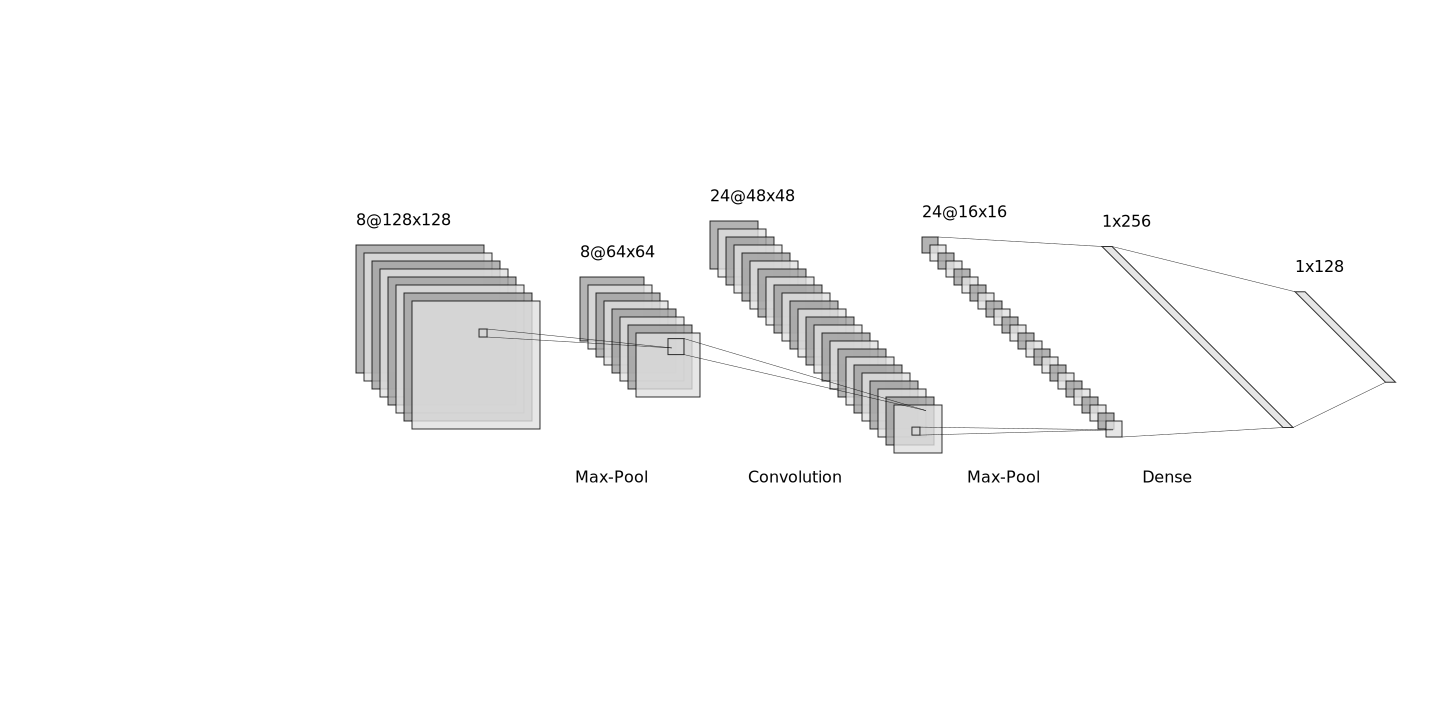
\includegraphics[width=\linewidth, bb=0 0 2000 572]{lenet.pdf}
\caption[Ein einfaches \acrshort{cnn}.]{Ein einfaches \acrshort{cnn}. Abbildung erstellt über \url{http://alexlenail.me/NN-SVG/LeNet.html} (Abgerufen am 18.5.2021).}\label{fig:cnn}
\end{figure}

\Cref{fig:cnn} zeigt ein solches \acrshort{cnn} im schematischen Aufbau. Ähnlich zum Aufbau einer Retina, welche durch die rasterförmig angeordneten Rhodopsinrezeptoren einfallende Photonen detektiert, werden die Eingaben bei \acrshort{cnn}s typischerweise in Form eines zweidimensionalen Rasters übergeben. Innerhalb des \acrshort{cnn}s finden sich anschließend hauptsächlich zwei alternierende Schritte, \textit{Convolution} und \textit{Pooling}. Jede Convolution-Schicht besteht aus einer oder mehreren Schichten von \textit{Feature Maps} (in \Cref{fig:cnn} gekennzeichnet durch Rechtecke). Diese setzen sich zusammen aus Rastern von Neuronen. Mathematisch können Neuronen in Convolution-Schichten in drei Dimensionen lokalisiert werden, $i$ und $j$ für die Position des Neurons im Raster einer jeden Feature Map und $z$ für den Index der Feature Map. Bei der Prozessierung einer Convolution-Schicht werden die Eingabedaten an Position $i, j$ in $z$-Richtung durch jede Feature Map geleitet und mit den neuronalen Gewichtungen und Aktivierungsfunktionen verrechnet. Somit kann für jede Eingabe $x_{i, j}$ eine Ausgabe $y_{i, j, z}$ für jede Feature Map an Index $z$ berechnet werden. Anschließend wird eine Pooling-Operation durchgeführt, welche die Dimensionalität der Ausgaben $y_{i, j, z}$ reduziert und in die nächste Schicht des Netzwerkes überführt. Die Pooling-Operation wird hierbei normalerweise jedoch nicht über jede Ausgabe $y_{i, j, z}$ für jede Eingabe $x_{i, j}$ der nachfolgenden Schicht berechnet, sondern nur für die $n\times n$ umliegenden Neuronen um $i, j$. Die Analogie zur Physiologie von neuronalen Systemen zur visuellen Reizintegration wird hier wieder deutlich, denn dies repräsentiert die rezeptiven Felder, welche sich beispielsweise in der Retina wiederfinden. Während die Feature Maps in den ersten Schichten des Netzwerkes noch einfache Features erkennen sollen (bei Bildern z.B. Kanten, Ecken), wird durch die Verknüpfung dieser erkannten Features in den tieferen Schichten über die Pooling-Operation sukzessiv ein abstraktes Verständnis der Eingabewerte erstellt. Nach der letzten Schicht können dann die Ausgaben über einen Dense Layer in Label zur Klassifikation überführt werden.

\acrshort{cnn}s eignen sich jedoch nicht nur zur Klassifikation von Bildern. Auch andere Eingabedaten können mit \acrshort{cnn}s klassifiziert werden. Beispielsweise können auch Audiodaten mit \acrshort{cnn}s verarbeitet werden. Da es sich bei Audiodaten, wie auch bei den Sensordaten zur Verkehrsmittelerkennung, um Zeitliniendaten handelt, können hierfür dieselben Methoden angewandt werden. Neben einer geeigneten Faltung der Eingabe-Features oder einer geeigneten Dimensionalisierung der ersten Convolution-Schicht wie in \cite{chen_deep_2015} ist es beispielsweise auch möglich, die Zeitliniendaten in ein Spektrogramm zu überführen, um das generierte Spektrogramm anschließend als Bild klassifizieren zu lassen \cite{ravi_deep_2016}.

\subsection{Nachverarbeitung}

Die Nachverarbeitung (\textit{Postprocessing}) gliedert sich an die Interpretation der Daten durch das Machine-Learning-Modell an. Dass die Ausgaben von Machine-Learning-Modellen nicht immer korrekt sein müssen, wurde bereits in der Diskussion der Validierungsverfahren motiviert. Oft verbleibt ein Restfehler des Modells, der während des Trainings nicht eliminiert werden kann. Mit Betrachtung einer Verkehrsmittelerkennung auf Grundlage von Aktivitätsdaten bietet es sich beispielsweise an, die vorhergesagten Labels mit den Nachbarlabels abzugleichen (\textit{Smoothing} oder auch \textit{Healing}) und gegebenenfalls anzupassen. Hierüber kann eine weitere Verbesserung der Ergebnisqualität erzielt werden \cite{werner_kontinuierliche_2020}.
